\documentclass[11pt,a4paper,onecolumn,final]{article}

%OT1 is the default font encoding of memoir class
%It is generally advised to put it before inputenc
%\usepackage{kerkis}
\usepackage[T1]{fontenc}

%Input encoding for typing directly Greek characters
%Other values for the option: latin1, ascii, ansinew
%It is generally advised to put it before babel
\usepackage[utf8]{inputenc}

%MAIN Language the LAST one
\usepackage[greek,english]{babel}

%\usepackage{kerkis}

%The teubner package extends the facilities offered by the CB Greek fonts
%NOTE: This includes also the graphicx package!
%NOTE: When the teubner package is loaded, command \cap (denoting set intersection) is overwritten
%NOTE: TEUBNER.STY FILE HAS BEEN CHANGED A BIT IN LINES 255-257 WITH 3 REPLACEMENTS \cap -> \capt
\usepackage{teubner}

%Package for displaying math
\usepackage{amsmath}

%Loading a superset of amsfonts
\usepackage{amssymb}

%Provides an enhanced version of \newtheorem
%1.Defines * for unnumbered environments
%2.Defines a proof environment
%3.Defines plain, definition, and remark theorem styles
\usepackage{amsthm}

%Allows text in eps files to be replaced with LATEX symbols
\usepackage{psfrag}

%An extension of the cite package, compatible with the IEEEtranN bibliography style
\usepackage[numbers,sort&compress]{natbib}

\makeatletter\let\c@lofdepth\relax\let\c@lotdepth\relax\makeatother
\usepackage[small,bf,tight]{subfigure}

%Math symbols of the dsfont style. Enables the use of \mathds{}
\usepackage{dsfont}

%Defines several symbols in text mode (e.g. the \textreferencemark for use in the itemize environment)
\usepackage{textcomp}

%Enables the Ralph Smith's Formal Script font in math mode via the \mathscr{} command
\usepackage{mathrsfs}

\usepackage{geometry}
%PDF VIEW
\geometry{total={210mm,297mm},left=25mm,right=25mm,bindingoffset=0mm, top=25mm,bottom=25mm}
%PRINT
%\geometry{total={210mm,297mm},left=20mm,right=20mm,bindingoffset=10mm, top=25mm,bottom=25mm}

\usepackage[breaklinks=true,colorlinks=true,
%linkcolor=blue,urlcolor=blue,citecolor=blue,% PDF VIEW
linkcolor=black,urlcolor=black,citecolor=black,% PRINT
bookmarks=false,bookmarksopenlevel=2]{hyperref}
\usepackage{bm}

%Convenient language switch
\newcommand{\gr}[1]{\foreignlanguage{greek}{#1}}
\newcommand{\en}[1]{\foreignlanguage{english}{#1}}
\newcommand{\dmin}{d_\text{min}}

%\newtheorem{definition}{Ορισμός}
\newtheorem{definition}{Definition}
\newtheorem{example}{Example}
\newtheorem{exercise}{Exercise}
%\newtheorem{lemma}{Λήμμα}
\newtheorem{lemma}{Lemma}
%\newtheorem{proof}{Proof}
\newtheorem{notation}{Notation}
\newtheorem{problem}{Problem}
%\newtheorem{proposition}{Πρόταση}
\newtheorem{proposition}{Proposition}
\newtheorem{remark}{Remark}
\newtheorem{solution}{Solution}
\newtheorem{summary}{Summary}
\newcommand{\argmax}{\arg\!\max}
%\addto\captionsgreek{\renewcommand{\chaptername}{Κεφάλαιο}}
%\addto\captionsgreek{\renewcommand{\tablename}{Πίνακας }}
%\addto\captionsgreek{\renewcommand{\proofname}{Απόδειξη }}
\setlength{\parindent}{0pt}
\setcounter{section}{-1}
\graphicspath{{./media/}}

\makeatletter
%\renewcommand{\fnum@figure}{Σχήμα \thefigure}
%\renewcommand{\fnum@table}{Πίνακας \thetable}
\makeatother
\begin{document}

%COVER PAGE%%%%%%%%%%%%%%%%%%%%%%%%%%%%%%%%%%%%%%%%%%%%%%%%%%%%%%%%%%%%%%%%%%%%%
\thispagestyle{empty}
{\sffamily\centering\Large

\vspace{\fill}

{\Large Aristotle University of Thessaloniki\\
Department of Electrical and Computer Engineering\\
Telecommunications Division}\\[0.5cm]


\vspace{2.0cm}

{\LARGE Ioannis Dimoulios 10641 \\
        Dimitrios Diakoloukas 10642}

\vspace{3.5cm}


{\LARGE Communication Systems II}\\[1em]

{\Large Constellation Design for Simultaneous  Wireless Information and Power Transfer (SWIPT)}

\vspace{3.5cm}

%\vspace{\fill}

%
}
%%COVER PAGE%%%%%%%%%%%%%%%%%%%%%%%%%%%%%%%%%%%%%%%%%%%%%%%%%%%%%%%%%%%%%%%%%%%%%

\newpage


%ABSTRACT%%%%%%%%%%%%%%%%%%%%%%%%%%%%%%%%%%%%%%%%%%%%%%%%%%%%%%%%%%%%%%%%%%%%%%%
%\chapter*{Abstract}
%\en{In this paper...}
%ABSTRACT%%%%%%%%%%%%%%%%%%%%%%%%%%%%%%%%%%%%%%%%%%%%%%%%%%%%%%%%%%%%%%%%%%%%%%%

\newpage

%\tableofcontents


\section{Introduction}
The task requires the analysis and design of various constellations considering the
balance in simultaneous wireless information and power transfer (SWIPT) systems.
Specifically, the focus is on the relationship between peak-to-average power ratio (PAPR)
and minimum Euclidean distance ($d_{\text{min}}$) in designing optimal constellations for SWIPT and reviewing their performance in terms of symbol error rate (SER).

We examine known modulation schemes such as 16-PAM, 16-PSK, and 16-QAM, as well as the state of the art 16-Circular QAM (CQAM) and 16-Spike QAM (sQAM) as presented in \cite{cqam} and \cite{sqam} respectively. In the final sections of the assignment we propose a new modulation scheme, namely 16-Bee QAM (BQAM), which shows promising results. 

Our approach includes both a theoretical and a simulation analysis. Constellations are represented with simple arrays of complex numbers in Julia with the convention that the first two symbols of the array always have distance \(d_\text{min}\). A more thorough explanation of our software setup is included in the Appendix section.  


\section{PAPR versus \(d_\text{min}\)}
In what follows the average symbol energy for all the constellations is normalized on \(E_s = 1\). This ensures that the comparisons are fair energy-wise. Moreover, \(M = 16\) is the number of symbols for each constellation. 

\subsection{Theoretical Analysis}
\subsubsection*{16-PAM} 
Assume that the energy of the main pulse of the PAM is \(E_g\). It is well known that 
\begin{equation}
    E_g = \frac{3E_s }{M^2 - 1} = 0.0118. 
\end{equation}
Then, given that the symbol with the highest energy, i.e. the symbol furthest from the origin has coordinates 
\begin{equation}
    x_M = \left\{(M-1)\sqrt{E_g}\right\}, 
\end{equation}
we can calculate PAPR as follows 
\begin{equation}
    \text{PAPR}_\text{PAM} = \frac{|x_M|^2}{E_s} = 2.647.
\end{equation}
As far as the minimum euclidean distance is concerned, we have
\begin{equation}
    d_\text{min} = 2\sqrt{E_g} = 0.217.
\end{equation}

\begin{figure}[h]
    \centering
    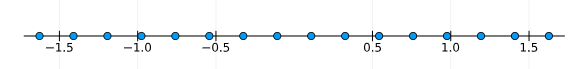
\includegraphics[scale=0.7]{16pam.png}
    \caption{16-PAM constellation diagram}
\end{figure}

\newpage

\subsubsection*{16-PSK}
The symbols of PSK have coordinates 
\begin{equation}
    x_i = \left\{ \sqrt{E_s}\cos \theta_i, \sqrt{E_s} \sin \theta_i \right\}
\end{equation}
where \(\theta_i = \dfrac{2\pi (i-1) }{M}\) for all \(i = 1, \ldots, M\). Hence for all \(i\), we have 
\begin{equation}
    E_i = |x_i|^2 = \sqrt{\cos ^2 \theta_i + \sin ^2 \theta_i} = 1,
\end{equation}
which in turn means \(E_\text{max}\) = 1 and
\begin{equation}
    \text{PAPR}_\text{PSK} = \frac{E_\text{max}}{E_s } = 1. 
\end{equation}
It also follows from simple trigonometric calculations that 
\begin{equation}
    d_\text{min} = 2\sqrt{E_s}\sin \frac{\pi}{M } = 0.390. 
\end{equation}

\begin{figure}[h]
    \centering
    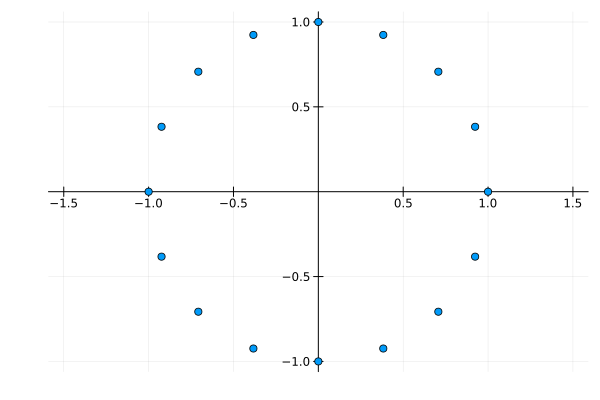
\includegraphics[scale=0.7]{16psk.png}
    \caption{16-PSK constellation diagram}
\end{figure}

\subsubsection*{16-QAM}
\(M\)-QAM is essentially the composition of two orthogonal \(\sqrt{M}\)-PAM constellations representing the I/Q components of the constellation. The energy is equally shared between each component; hence 
\begin{equation}
    E_s = 2E_{s\left(\sqrt{M}-\text{PAM}\right)}
\end{equation}
and if \(E_g\) is the energy of the main pulse of each \(\sqrt{M}\)-PAM component we have
\begin{equation}
    E_g = \dfrac{3E_{s\left(\sqrt{M}-\text{PAM}\right)}
}{\sqrt{M}^2 - 1} = \dfrac{1.5E_s }{M - 1} = 0.1.
\end{equation}
Then the coordinates of the symbol with the highest energy are 
\begin{equation}
    x_M = \left\{ \left(\sqrt{M} - 1\right)\sqrt{E_g}, \left(\sqrt{M} - 1\right)\sqrt{E_g} \right\}. 
\end{equation}
Now, we can calculate 
\begin{equation}
    \text{PAPR}_\text{QAM} = \frac{|x_M|^2 }{E_s } = 0.1\cdot 2 \cdot 3^2 = 1.8.
\end{equation}
On the other hand 
\begin{equation}
    d_\text{min} = 2\sqrt{E_g} = 0.632.
\end{equation}
\begin{figure}[h]
    \centering
    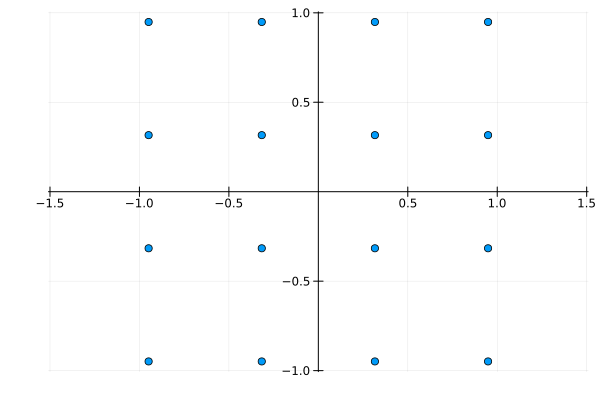
\includegraphics[scale=0.7]{16qam.png}
    \caption{16-QAM constellation diagram}
\end{figure}

\subsubsection*{16-CQAM}
According to the algorithm provided \cite{cqam} we initialize CQAM as a function of two parameters: 
\begin{itemize}
    \item \(N\), the number of circles of the constellation and
    \item \(d_\text{min}\), the minimum euclidean distance, from which we can directly calculate the radius of the first circle. 
\end{itemize}
Each circle must contain \(n = M \div N \) symbols. Indeed, the first radius is 
\begin{equation}
    R_1 = \frac{d_\text{min} }{2\sin \frac{\pi}{ n}}.
\end{equation}\\ 
Next, we create the first circle with \(n \) symbols such that adjacent symbols are distanced at \(d_\text{min}\). 

The next \(N-2\) circles are formed with \(n\) with the minimum possible radius such that the \(d_\text{min}\) condition is not violated. 

The remaining energy is then used to form the last circle with radius \(R_N > R_j\) \\ for all \(j \in 1,\ldots , N-1\).

Hence, considering that the symbols carrying the maximum energy are those of the last circle we can calculate,  
\begin{equation}
    \text{PAPR}_\text{CQAM} = \frac{R_N^2}{E_s } = R_N^2. 
\end{equation}
In order to create these constellations on software, we used rotating vectors of modulus \(d_\text{min}\) to form equilateral triangles on the first \(N-1\) circles. The results are presented in the diagram below. 

\begin{figure}[h]
    \centering
    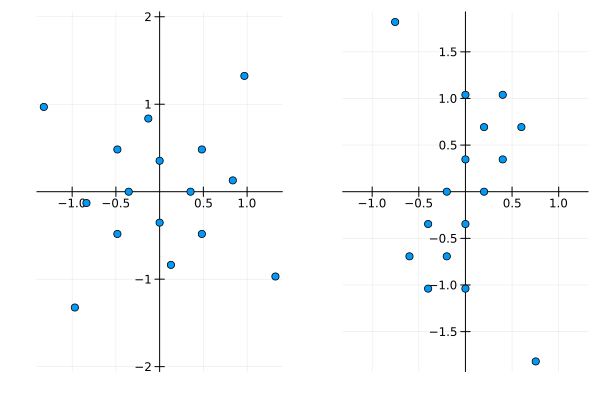
\includegraphics[scale=0.7]{16cqam_dual.png}
    \caption{16-CQAM constellations, a) with \(N=4\), \(\dmin = 0.5\)} and b) with \(N=8\), \(\dmin = 0.4\)
\end{figure}

\newpage
\subsection{Simulation Results}
For PAPR calculations, we used the normalized average \(E_s = 1\) for each constellation and found the symbol with maximum energy by means of linear search. 

For \(\dmin \) calculations we made sure we adhered to the convention stated in the introduction, namely that the first two symbols of the constellation are distanced at \(\dmin\). 

The simulations are therefore summarized in the following figure. 

\begin{figure}[h]
    \centering
    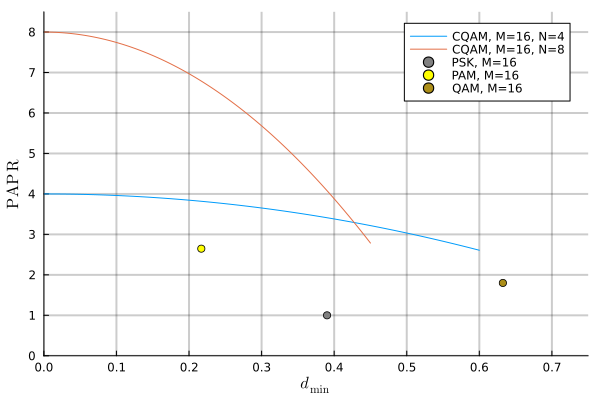
\includegraphics[scale=0.7]{ex1_sim.png}
    \caption{PAPR versus \(\dmin \) plot for various modulation schemes}
\end{figure}

Notice that the PSK point differs from the one presented in \cite{cqam}. Additionally, there is a slight variation for both the CQAM curves compared to \cite{cqam}. 
% Unfortunately, we could not get the exact results demonstrated in the paper. 



\bibliographystyle{IEEEtranN}
\en{\bibliography{sample}}

\end{document}